%%
%% Author: dariochinelli
%% 2021-04-05
%%


\section{Cross section}
Quando una radiazione elettromagnetica interagisce con la materia sono quattro i processi che consideriamo: \\
\textbf{Effetto fotoelettrico}: assorbimento totale del fotone \\
\textbf{Produzione di coppie}: assorbimento totale del fotone \\
\textbf{Scattering di Rayleigh}: diffusione del fotone in cui non perde energia \\
\textbf{Effetto Compton}: diffusione del fotone in cui perde energia \\
La cross section rappresenta la probabilità che questi effetti avvengono.

\paragraph{Ad esempio} per l'effetto fotoelettrico la cross section è:
\begin{equation}
\begin{split}
& \sigma_{PE} \quad \mbox{sezione d'urto fotoelettrica} \\
& N_{PE} = \sigma_{PE} I n
\end{split}
\end{equation}
Dove $I$ è il numero di fotoni del fascio incidente sulla lamina, $n$ è il numero di atomi per unità di area e quindi $N_{PE}$ definisce il \textbf{numero di processi di assorbimento fotoelettrico}.
Se la lamina la assumo molto sottile, posso affermare che gli atomi non si "schermino" tra loro.
La sezione d'urto mi esprime quanto \textit{efficacemente} i fotoni vengono assorbiti dalla lamina.
$\sigma_{PE}$ deve quindi avere le dimensioni di un'area.
Possiamo dare un'interpretazione geometrica alla probabilità, dove considero un cerchio di area $\sigma_{PE}$ intorno al nucleo per cui ogni fotone che si avvicina entrando dentro questo cerchio interagisce con l'atomo.
\begin{figure}[h]
\centering
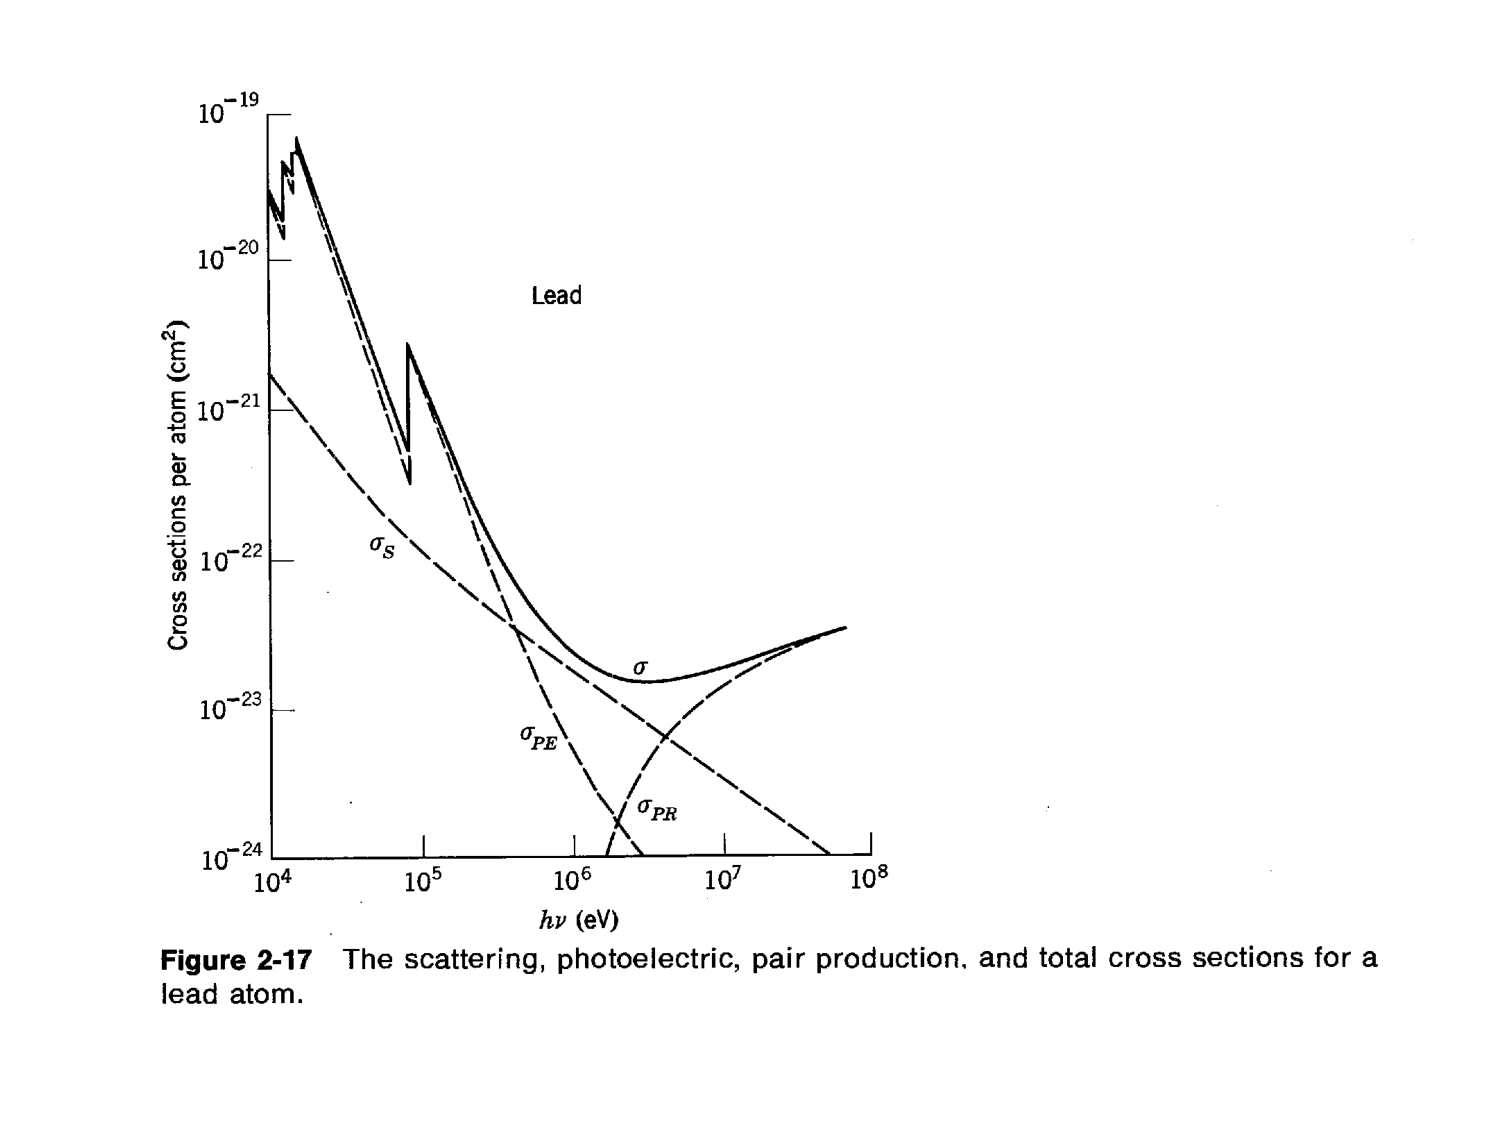
\includegraphics[scale=0.5]{/cross_section}
\caption{Cross section del Piombo (Lead). Si vede la cross section in funzione dell'energia del fotone. La linea continua rappresenta la \textbf{cross section totale} e linee tratteggiate sono le cross section riferite ai singoli processi. $\sigma_S$ rappresenta lo scattering e somma la diffusione alla Rayleigh e diffusione alla Compton. $\sigma_{PR}$ cross section produzione di coppie. $\sigma_{PE}$ effetto fotoelettrico.}
\end{figure}

Notare che i picchi nella curva di $\sigma_{PE}$ sono dovuti e corrispondono alle diverse energie di legame nell'atomo di piombo.
Quando l'energia del fotone diventa più piccola dell'energia di legame non avviene più effetto fotoelettrico, si definiscono quindi delle \textit{soglie}.





